\documentclass[11pt,a4paper]{scrartcl}
\typearea{12}
\usepackage{graphicx}
\usepackage{pstricks}
\usepackage{listings}
\usepackage{amsmath}
\usepackage{tikz}
%\usepackage{tikzscale}
%\usepackage{pgfplots}

\newcommand{\ms}{\mbox{\,ms}}
\newcommand{\mV}{\mbox{\,mV}}
\newcommand{\kHz}{\mbox{\,kHz}}
%\pgfplotsset{compat=1.8}


\usepackage{fancyhdr}
\pagestyle{fancy}
\lfoot{\texttt{github.com/conorhoughton/COMS30127}}
\lhead{Computation Neuroscience - 14\_phase\_analysis (j/k) - Conor}
\rhead{\thepage}
\cfoot{}

\begin{document}

\section*{Phase analysis}
To recap, we have seen the Hodgkin Huxley equation
\begin{equation}
C_m\frac{dV}{dt}=g_{\text{\l}}(E_{\text{\l}}-V)+g_{\text{Na}}(E_{\text{Na}}-V)+g_{\text{K}}(E_{\text{K}}-V)+I
\end{equation}
where the sodium and potassium conductances, $g_{\text{Na}}$ and
$g_{\text{K}}$ have complicated non-linear dynamics. In fact, the
Hodgkin-Huxley equation is really four equation, an equation for $V$
along with equations for the three gating variables $n$, $m$ and $h$, each of the form
\begin{equation}
\frac{dk}{dt}=\alpha_k(1-k)-\beta_k k
\end{equation}
with $k$ standing in for $n$, $m$ or $h$ and $\alpha_k(V)$ and $\beta_k(V)$
being the probability of going from closed to open and open to
closed. By moving stuff around this can be easily rewritten in a familiar form
\begin{equation}
\tau_k\frac{dk}{dt}=k_\infty - k
\end{equation}
with 
\begin{equation}
\tau_k=\frac{1}{\alpha_k+\beta_k}
\end{equation}
and
\begin{equation}
k_\infty=\frac{\alpha_k}{\alpha_k+\beta_k}
\end{equation}
Hence the ion channels relax towards some asymptotic value $n_\infty$,
$m_\infty$ and $h_\infty$ with some time scale $\tau_n$, $\tau_m$ and
$\tau_h$; however all these quantities depend on the voltage so the
equations are coupled to the voltage equation.

This is a complicated non-linear equation; in fact, real neurons are
likely to be even more complicated. As was mentioned before; the
Hodgkin-Huxley equation as described here describes the voltage
dynamics of the squid giant axon. The same name is often used to
describe the more complex versions of these models
\begin{equation}
C_m\frac{dV}{dt}=\mbox{lots of different ionic currents}
\end{equation}
used to describe real neurons. These typically include other channels,
often more than one potassium channel which adds other timescales to
the dynamics, calcium channels which play some of the same role as the
sodium channels, other sodium channels with more complex dynamics,
calcium-gated potassium channels whose open and closing depends not on
the voltage but on the concentration of calium ions, and so on. All of
this complexity emphasises the neuron itself as a site of computation,
rather than as a node in a network. As such, it is important to
understand the dynamics of the neurons models, however, their
complexity makes this hard and so we start not by allowing the
Hodgkin-Huxley model to become more complex, but by simplifying it.

When it is recognized as a system of four non-linear differential
equation it is clear that it may prove hard to analyse the
Hodgkin-Huxley equation; for example, the phase space is
four-dimensional for a start, making it hard to picture. For this
reason it is common to simplify the Hodgkin-Huxley equation in the
hope of getting some insight into its behaviour, this is important,
for example, if you are interested in getting an intuitive
understanding of how different neuronal models can support the
different behaviours of observed in neurons: some neurons spike
continuously, some don't; some burst, that is, switch back and forth
between high spiking and low spiking states.

The goal then is look at models that approximate the Hodgkin-Huxley
equation and simplify while keeping it complex enough so that it is
still a rich enough to model spiking.

\subsection*{The Morris-Lecar model}


Morris and Lecar  \cite{MorrisLecar1981} developed their model in a direct way as a good model
of the dynamics of a muscle fibre in the barnacle.  However, just as
the Hodgkin-Huxley model is a model of a specific axon, the squid
giant axon, that is adapted to wider use, the Morris-Lecar is a model
of a muscle fibre in the barnacle. Like Hodgkin and Huxley, they wrote
down an equation of the form they expected to work and then adjust
parameters to fit the actual data. Here, however, we will talk about
the way this model could approximate the Hodgkin-Huxley model.

The key idea is that $\tau_m$ is very small. When we looked at the
behaviour of equations like the equation for $m$ we saw that the
functions track their asymptotic value, with the $\tau$ value
governing how closely it succeeds in reaching the equilibrium
situation where $m$ equals $m_\infty$. Since $\tau_m$ tends to be very
small, often less than a milisecond, it is reasonable to replace $m$
by $m_\infty$. Next the effect of $h$ is ignored, or lumped in with
$n$, in short, from a mathematical point of view stopping the influx
of sodium ions and increasing the flow of potassium is similar to
allowing the sodium ions to continue flowing inwards while increasing
the potassium flow even more.

Altogether this gives a two-dimensional model of the neuron which is
much easier to think about.  The model is simplified further by
ignoring the indices on the gating variables, so the single gating
variable appears with a single power. The sub-gate structure of ion
channels gives a very sharp response curve, with gating variables like
$m$ and $n$ changing rapidly from near zero to near one; however, a
similar behaviour can be introduced mathematically by just changing
the shape of the asymptotic value.

In the barnacle the main ion responsible for depolarization is calcium
rather than by sodium, so the model has calcium rather than sodium, in
applying the model to other neurons this could be changed but here we
will describe the channel with a positive reversal potential as a
calcium channel.

The Morris-Lacer model is
\begin{equation}
\tau_m\frac{dV}{dt}=E_{\text{l}}-V+R_mg_{\text{Ca}}m_\infty(E_{\text{Ca}} -V)+R_mg_{\text{K}}n(E_{\text{K}} -V)+R_mI
\end{equation}
and
\begin{equation}
\tau_n\frac{dn}{dt}=n_\infty-n
\end{equation}
where
\begin{eqnarray}
m_\infty&=&\frac{1}{2}\left(1+\tanh\left[\frac{V-V_1}{V_2}\right]\right)\cr
n_\infty&=&\frac{1}{2}\left(1+\tanh\left[\frac{V-V_3}{V_4}\right]\right)\cr
\tau_n&=&1/\left(\phi\cosh\left[\frac{V-V_3}{2V_4}\right]\right)
\end{eqnarray}
Obviously there are lots of parameters here, and changing the
parameters changes the behaviour of the model; a set of typical values would be
$\tau_m=10\ms$, $R_mg_{\text{Ca}}=2$, $E_{\text{Ca}}= 120\mV$, $R_mg_{\text{K}}= 8$, $E_{\text{K}}=-84\mV$,$V_1=-1.2\mV$,$V_2= 18\mV$,$V_3= 2\mV$,$V_4= 30\mV$,$\phi= 0.04\kHz$.

Now, to understand how this equation works we will examine the
nullclines, the lines where the derivatives are zero:
$dV/dt=dn/dt=0$. These nullclines are easily found, they are
\begin{equation}
n=-\frac{E_{\text{l}}-V+R_mg_{\text{Ca}}m_\infty(E_{\text{Ca}} -V)+R_mI}{R_mg_{\text{K}}(E_{\text{K}} -V)}
\end{equation}
for the $v$-nullcline and 
\begin{equation}
n=n_\infty
\end{equation}
for the $n$-nullcline. The key point is that the $V$-nullcline has a
sort of cubic shape which for many parameter values is cut by the
$n$-nullcline, an example is given in Fig.~\ref{ML_phase}.

\begin{figure}
\begin{center}
  
  \setlength{\unitlength}{0.0500bp}%
  \begin{picture}(8820.00,3024.00)%

      \put(176,2900){{\makebox(0,0){\strut{}\textbf{A}}}}%
        \put(4676,2900){{\makebox(0,0){\strut{}\textbf{B}}}}%     

      \put(946,704){\makebox(0,0)[r]{\strut{} 0}}%
      \put(946,1128){\makebox(0,0)[r]{\strut{} 0.2}}%
      \put(946,1552){\makebox(0,0)[r]{\strut{} 0.4}}%
      \put(946,1975){\makebox(0,0)[r]{\strut{} 0.6}}%
      \put(946,2399){\makebox(0,0)[r]{\strut{} 0.8}}%
      \put(1328,484){\makebox(0,0){\strut{}-50}}%
      \put(1951,484){\makebox(0,0){\strut{}-25}}%
      \put(2575,484){\makebox(0,0){\strut{} 0}}%
      \put(3074,484){\makebox(0,0){\strut{} 20}}%
      \put(3823,484){\makebox(0,0){\strut{} 50}}%
      \put(176,1731){\rotatebox{-270}{\makebox(0,0){\strut{}$n$}}}%
      \put(2500,154){\makebox(0,0){\strut{}$V$ (mV)}}%

    \put(0,0){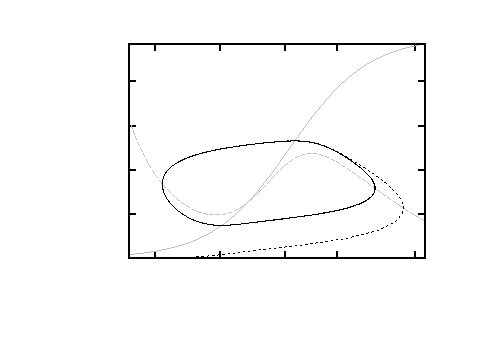
\includegraphics{60_phase}}%


      \put(5314,1196){\makebox(0,0)[r]{\strut{}-25}}%
      \put(5314,1750){\makebox(0,0)[r]{\strut{} 0}}%
      \put(5314,2192){\makebox(0,0)[r]{\strut{} 20}}%
      \put(5446,484){\makebox(0,0){\strut{} 0}}%
      \put(6190,484){\makebox(0,0){\strut{} 0.25}}%
      \put(6935,484){\makebox(0,0){\strut{} 0.5}}%
      \put(7679,484){\makebox(0,0){\strut{} 0.75}}%
      \put(8423,484){\makebox(0,0){\strut{} 1}}%
      \put(4676,1731){\rotatebox{-270}{\makebox(0,0){\strut{}$V$ (mV)}}}%
      \put(6934,154){\makebox(0,0){\strut{}$t$ (s)}}%

    \put(4500,0){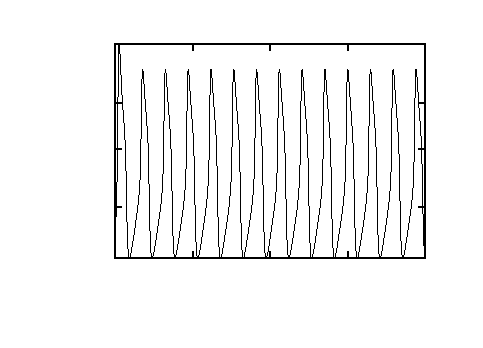
\includegraphics{60_trace}}%


  \end{picture}%


\end{center}
\caption{This shows the phase space for the Morris-Lecar equation, it is a temporary figure taken from DOI10.1007/s002850050157 which uses a lower case $v$ for $V$ and uses $w$ where we use $n$. \label{ML_phase}}
\end{figure}


\begin{figure}
\begin{center}

  \setlength{\unitlength}{0.0500bp}%
  \begin{picture}(8820.00,3024.00)%

      \put(176,2900){{\makebox(0,0){\strut{}\textbf{A}}}}%
        \put(4676,2900){{\makebox(0,0){\strut{}\textbf{B}}}}%     

      \put(946,704){\makebox(0,0)[r]{\strut{} 0}}%
      \put(946,1128){\makebox(0,0)[r]{\strut{} 0.2}}%
      \put(946,1552){\makebox(0,0)[r]{\strut{} 0.4}}%
      \put(946,1975){\makebox(0,0)[r]{\strut{} 0.6}}%
      \put(946,2399){\makebox(0,0)[r]{\strut{} 0.8}}%
      \put(1328,484){\makebox(0,0){\strut{}-50}}%
      \put(1951,484){\makebox(0,0){\strut{}-25}}%
      \put(2575,484){\makebox(0,0){\strut{} 0}}%
      \put(3074,484){\makebox(0,0){\strut{} 20}}%
      \put(3823,484){\makebox(0,0){\strut{} 50}}%
      \put(176,1731){\rotatebox{-270}{\makebox(0,0){\strut{}$n$}}}%
      \put(2500,154){\makebox(0,0){\strut{}$V$ (mV)}}%

    \put(0,0){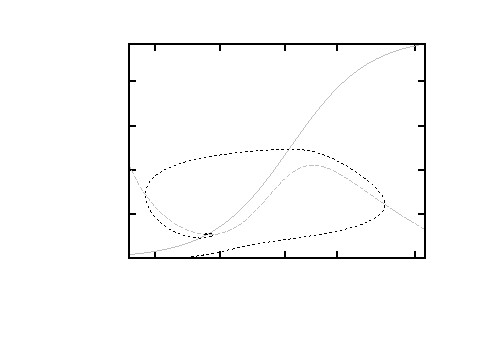
\includegraphics{40_phase}}%


      \put(5314,1196){\makebox(0,0)[r]{\strut{}-25}}%
      \put(5314,1750){\makebox(0,0)[r]{\strut{} 0}}%
      \put(5314,2192){\makebox(0,0)[r]{\strut{} 20}}%
      \put(5446,484){\makebox(0,0){\strut{} 0}}%
      \put(6190,484){\makebox(0,0){\strut{} 0.25}}%
      \put(6935,484){\makebox(0,0){\strut{} 0.5}}%
      \put(7679,484){\makebox(0,0){\strut{} 0.75}}%
      \put(8423,484){\makebox(0,0){\strut{} 1}}%
      \put(4676,1731){\rotatebox{-270}{\makebox(0,0){\strut{}$V$ (mV)}}}%
      \put(6934,154){\makebox(0,0){\strut{}$t$ (s)}}%

    \put(4500,0){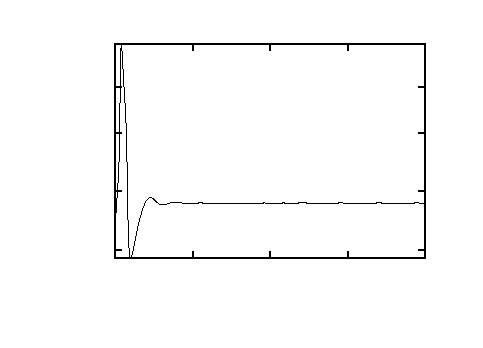
\includegraphics{40_trace}}%


  \end{picture}%


\end{center}
\caption{This shows the phase space for the Morris-Lecar equation, it is a temporary figure taken from DOI10.1007/s002850050157 which uses a lower case $v$ for $V$ and uses $w$ where we use $n$. \label{ML_phase}}
\end{figure}


It is possible to understand different spiking regimes from this
figure. Remember the nullclines separate areas with different signs
for $dV/dt$ and $dn/dt$, to the left of the $dn/dt$ nullcline $n$
increases, to the right it decreases, above the $dV/dt$ nullcline $V$
decreases, below it, it increases. In Fig.~\ref{ML_phase}A there is a
single equilibrium point where the two lines cross, but it is easy to
see from the arrow directions that this is unstable, in fact there is
a limit cycle and the equation with this phase diagram exhibits
regular spiking, this is shown in Fig.~\ref{ML_spike}. In
Fig.~\ref{ML_phase}B the equilibrium point is stable so this time the
model does not spike regularly, however if the system is moved away
from the equilibrium point it sometimes returns there by spiking.


\begin{figure}
\begin{center}
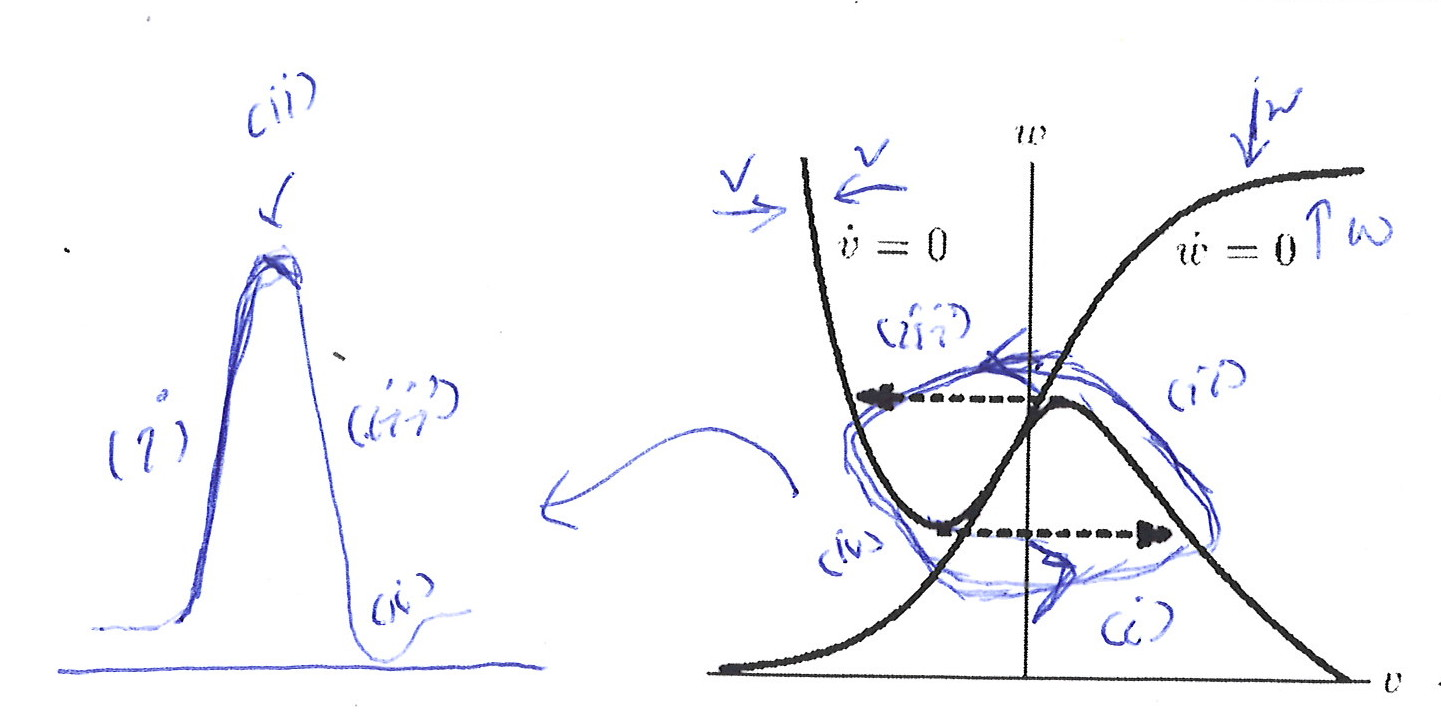
\includegraphics[width=8cm]{ML_spike.jpg}
\end{center}
\caption{This is a sketch for the Morris-Lecar limit cycle. \label{ML_spike}}
\end{figure}

\subsection*{FitzHugh-Nagumo model}

One advantage of the FitzHugh-Nagumo model
\cite{FitzHugh1955,Nagumo1962} is that it is clear how it derived from
the Hodgkin-Huxley equation, though a formal derivation yields
slightly different results. However, one disadvantage is that the
actual mathematical form of the equations is quite
complicated. Although its origin is quite different one way to think
of the FitzHugh-Nagumo model is as a model that has a similar phase
plane as the Morris-Lecar, but a much simpler form. The
FitzHugh-Nagumo model is
\begin{eqnarray}
\frac{dw}{dt}&=&v-\frac{1}{3}v^3-w+I\cr
\tau\frac{dw}{dt}&=&v+a-bw
\end{eqnarray}
where a little-v, $v$, has been used for the voltage to show these
quantities shouldn't be take seriously as biologically relevant, they
have been scaled to, for example, get rid of one of the time
constants. 

In this case we can solve the nullclines easily, the $v$-nullcline is
\begin{equation}
w=v+\frac{1}{3}v^3+I
\end{equation}
and the $w$-nullcline
\begin{equation}
w=\frac{v+a}{b}
\end{equation}
We see clearly that the $v$-nullcline has the same cubic shape as is
the case of the Morris-Lecar, the $w$-nullcline is a straight line
now, before it was a sort of sigmoid shape, but it has the same
property of crossing the $v$-nullcline at exactly one place. This gives a similar limit cycle as before: Fig.~\ref{FHN_phase}.



\begin{figure}
\begin{center}
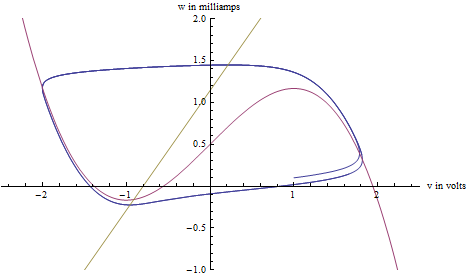
\includegraphics[width=8cm]{FHN_phase.png}
\end{center}
\caption{This is a graph of the FitzHugh-Nagumo phase plane with a limit cycle. The parameter values $I=0.5$, $a=0.7$, $b=0.8$, and $\tau=12.5$ and the figure is taken from Wikipedia.\label{FHN_phase}}
\end{figure}

In this model we can see the effect of changing $I$, it shifts the
$v$-nullcline up and down, as it does so it moves the equilibrium
point from stable to unstable and therefore shifts the model from
spiking to quite. There is nice animation of this available at\\
\\
\texttt{www.scholarpedia.org/article/FitzHugh-Nagumo\_model}. \\

One application of this is the study of bursting cells and pattern
generation; these are cells that send out regular burst of neurons;
these dynamics are important in controlling some fundamental
physiological systems where patterns are important, chewing in slugs,
struggling in tadpoles and so on. For this to work there is a slow
current, for example, a potassium current, whose effect is to reduce
$I$. The slow current sharply increases every time there is a spike and
then decays away slowly and these dynamics are considered slow enough
that it can be treated separately to the dynamics of $v$ and $w$. This
means that as the neuron spikes $I$ is decreased because of the
increase in the potassium current, eventually this cause the
equilibrium point to shift from an unstable point to a stable on and
spiking stops; it doesn't start again until the potassium current decays away.

\begin{thebibliography}{99}
\bibitem{MorrisLecar1981}
\newblock Morris, C and Lecar, H (1981),
\newblock Voltage Oscillations in the barnacle giant muscle fibre
\newblock Biophys. J., 35:93--213

\bibitem{FitzHugh1955}
\newblock FitzHugh R. (1955) 
\newblock Mathematical models of threshold phenomena in the nerve membrane. 
\newblock Bull. Math. Biophysics, 17:257--278

\bibitem{Nagumo1962}
\newblock Nagumo J., Arimoto S., and Yoshizawa S. (1962) 
\newblock An active pulse transmission line simulating nerve axon. 
\newblock Proc. IRE. 50:2061--2070.

\end{thebibliography}

\end{document}

